\documentclass[final,t]{beamer}

% poster template
\usepackage[orientation=portrait,size=a0,scale=1.4,debug]{beamerposter}
\usetheme{es}
\usepackage[utf8]{inputenc}
\usepackage{fontspec}
\usepackage{fontawesome}
\usepackage{color}
\usepackage{natbib}

% document properties
\title{Ecotoxicology is not normal.}
\author{Eduard Sz\"ocs, Ralf B. Sch\"afer}
\institute{Institute for Environmental Sciences, University Koblenz-Landau}
\footer{Paper, poster \& source code here: \color{black}{https://github.com/EDiLD/usetheglm}}


%------------------------------------------------------------------------------
\begin{document}
\begin{frame}{}
\begin{columns}[t]
%-----------------------------------------------------------------------------
%                                                                     COLUMN 1
% ----------------------------------------------------------------------------
\begin{column}{.48\linewidth}

    % Problem
    \begin{exampleblock}{Most eco(toxico)logical data is not normally distributed}
        \begin{center}
          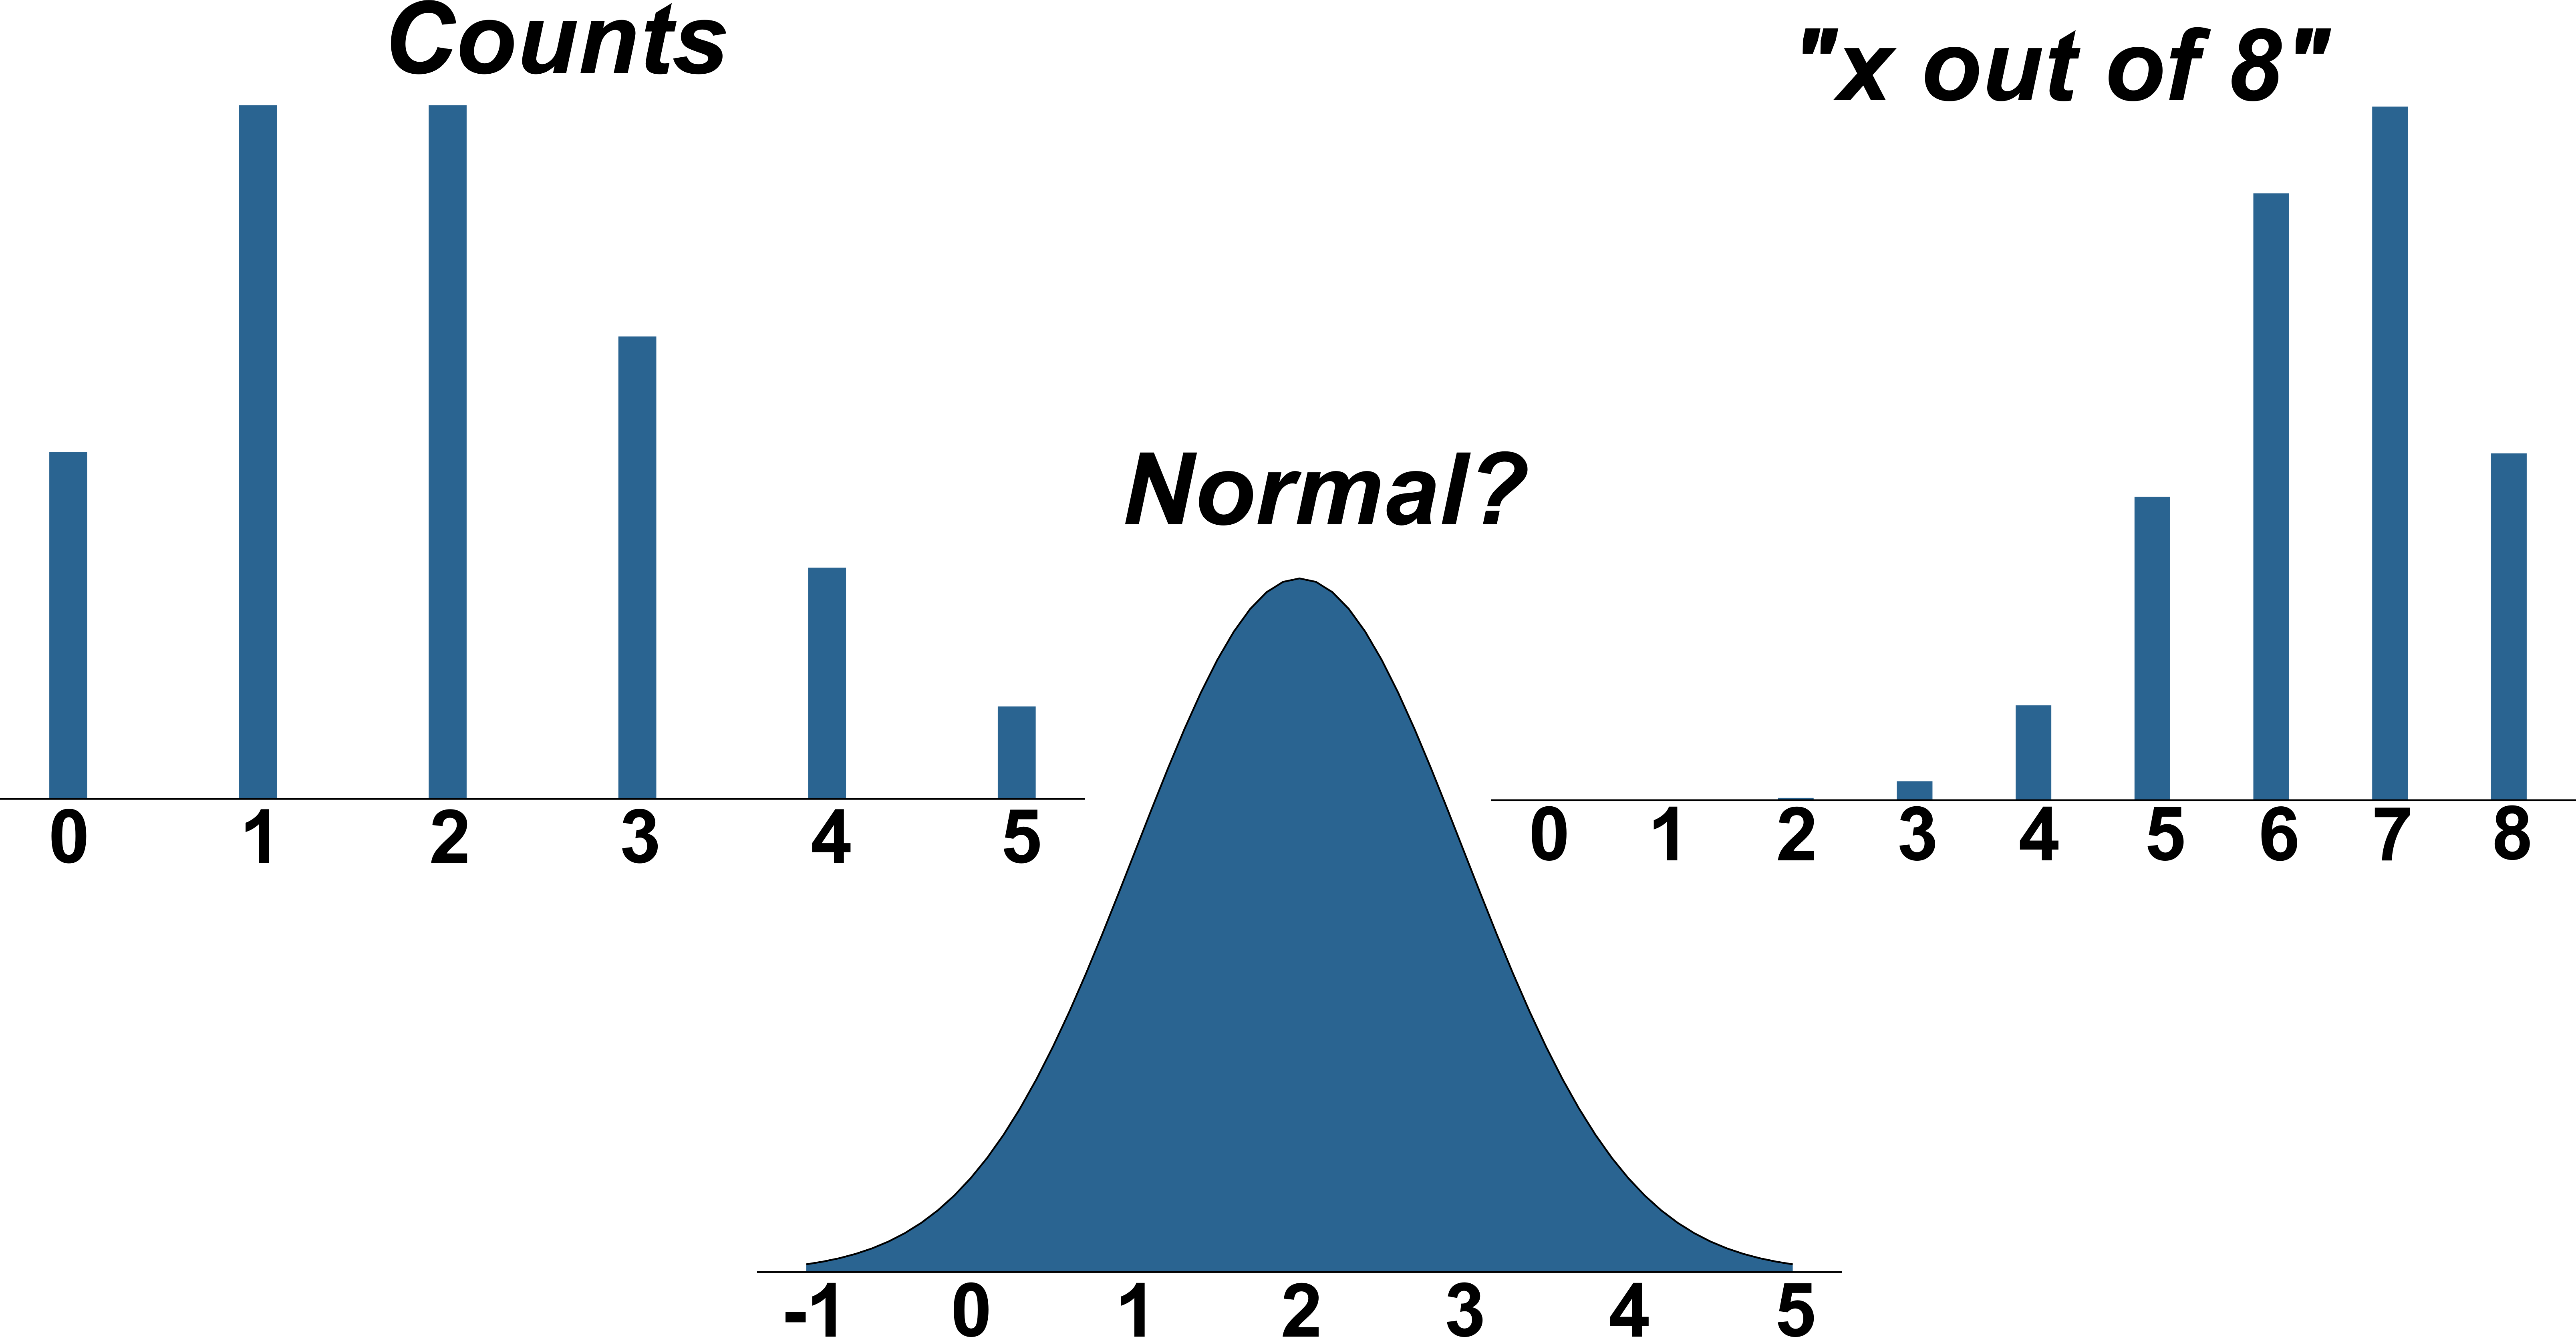
\includegraphics[width=0.7\linewidth]{fig/distr.png}
        \end{center}

        \begin{itemize}
            \item Usually analysed by \\[0.5ex]
                \begin{itemize}
                    \item transforming data (e.g. $log(Ax + C)$, $x^{0.5}, arcsine~x^{0.25}$) for linear model \cite{newman_quantitative_2012}
                    \item non-parametric methods \cite{wang_making_2011}
                \end{itemize}
            \item \emph{Generalized Linear Models} (GLM) an alternative to direct model such data
            \item Can GLMs enhance inference in ecotoxicology?
        \end{itemize}
    \end{exampleblock}


    \begin{block}{Methods: Simulation study}
    \begin{columns}[T]
    \begin{column}{.48\linewidth}
        \begin{itemize}
            \item Simulated count and binomial data
            \item One-factorial design
            \item Benchmarks:
                \begin{itemize}
                    \item  Power
                    \item Type I error
                \end{itemize}
            \item Variates:
                \begin{itemize}
                    \item Number of replicates
                    \item Abundance
                    \item Effect size
                    \item Methods 
                \end{itemize}
            \item Endpoints:
                \begin{itemize}
                    \item Global Treatment effect
                    \item LOEC
                \end{itemize}
            \end{itemize}
        \end{column}
        \begin{column}{.48\linewidth}
            \begin{figure}
             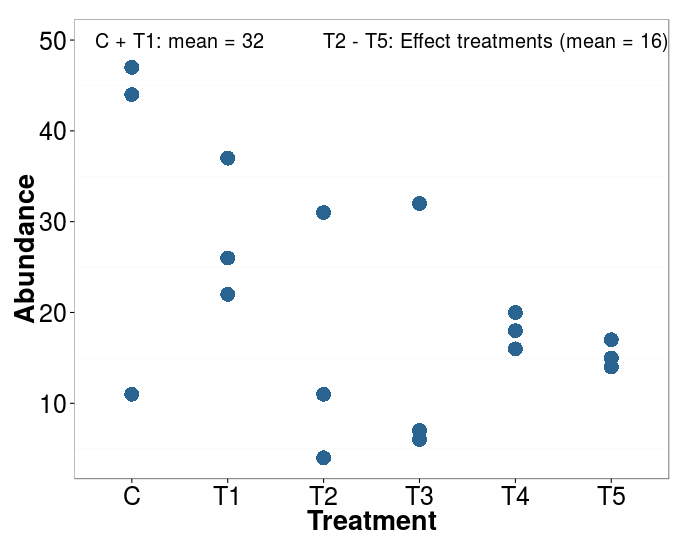
\includegraphics[width=.9\linewidth]{fig/sim.png}
             \caption{A realised simulation. N = 3, mean  = 32, effectsize = 50\%}
             \end{figure}
        \end{column}
        \end{columns}
    \end{block}

    \begin{block}{Results: Type I errors}
    \end{block}

\end{column}


%-----------------------------------------------------------------------------
%                                                                     COLUMN 2
% ----------------------------------------------------------------------------
\begin{column}{.48\linewidth}

    \begin{block}{Results: Power}
    \end{block}


    \begin{block}{Power estimation app}
    \begin{itemize}
        \item \emph{For "a priori"} power calculations
        \item web based, easy to use, for one factorial designs
        \item Currently hostet at \faGlobe~\textbf{\textcolor{blue}{http://52.28.43.83/shinypower/}}
    \end{itemize}
        \begin{center}
          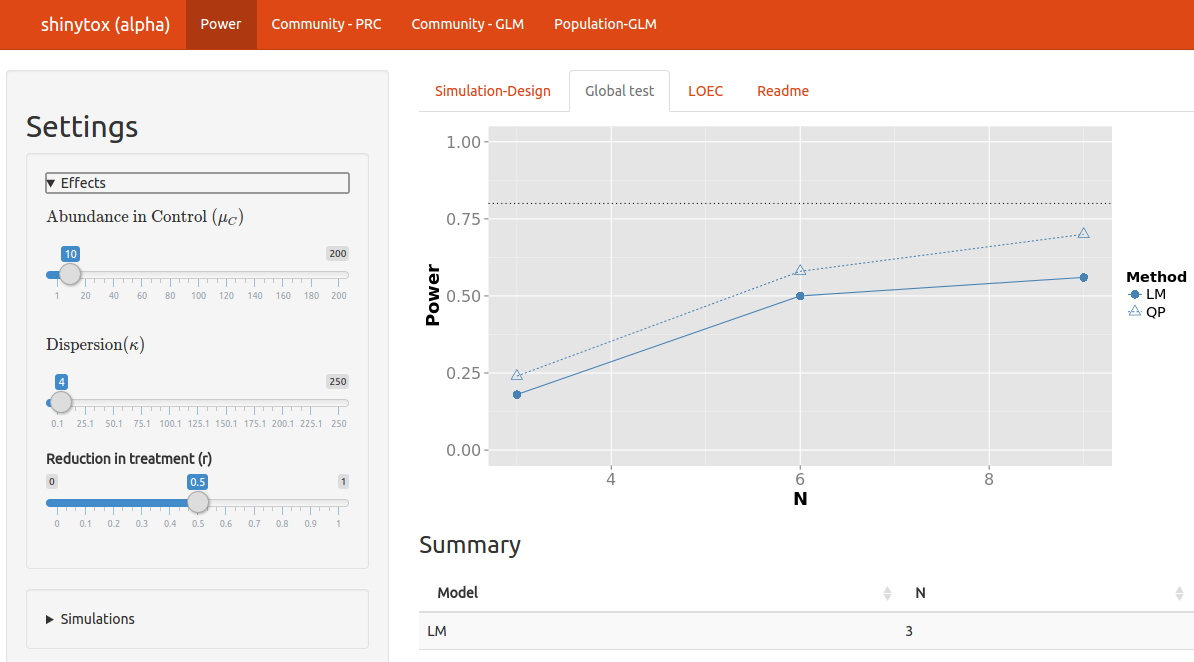
\includegraphics[width=0.7\linewidth]{fig/shinytox.png}
        \end{center}
    \end{block}
  
    % Conclusions
    \begin{alertblock}{Conclusions}
        \begin{itemize}
            \item Low power at common experimental designs (NOEC!?)
            \item Change your model, not your data!
            \item Negative binomial GLM not recommended (but see bootstrap).
        \end{itemize}
    \end{alertblock}

        % References
    \begin{block}{References}
        \vskip -0.8cm
        \footnotesize      
        \bibliographystyle{plain}
       \bibliography{references}    % i.e. the poster.bib file
        \vskip -0.8cm
    \end{block}

    \begin{block}{Contact}
    \vskip -0.5cm
    \normalsize
    \faEnvelope ~szoecs@uni-landau.de \hfill  \faTwitter ~@EduardSzoecs \\[1ex]
    \faGlobe ~http://edild.github.io/   \hfill \faGithub ~ @EDiLD
    \end{block}

\end{column}
\end{columns}

\end{frame}
\end{document}
